\chapter[A Parameter Space Exploration of Dust Formation]{A Parameter Space Exploration of Dust Formation within WCd Systems Using an Advected Scalar Dust Model}


\begin{abstract}
    
\end{abstract}

\section{Introduction}

Binary systems with colliding stellar winds are a fascinating phenomena capable of producing a variety of phenomena.
The shocks produced from these interacting systems create some of the most luminous persistent stellar-mass X-ray sources in the night sky \parencite{usov_stellar_1991}.
Within the wind collision region the available mechanical energy rivals the radiative energy of many stars, producing shocks with temperatures up to $10^8$ \si{\kelvin}.

Despite this, in particularly energetic Colliding Wind Binary (CWB) systems, such as those with an evolved Wolf-Rayet (in particular the WC sub-type) star as the source of the dominant wind in the system (A WR+OB binary), dust has been observed to form.
\textcite{allenInfraredPhotometryNorthern1972} first attributed IR excess around WC systems to dust in the form of amorphous carbon grains; however, the high wind temperatures and extremely high luminosities around WC systems are such that dust grains would be readily destroyed through sublimation processes.
Despite this, dust has been observed to form readily in binary systems ( a WCd system), despite an additional highly luminous star and shocks that would quickly destroy dust acting upon these nascent, fragile dust grains.
The exact mechanisms of dust formation as well as the evolution of dust within these systems is poorly understood.
However dust formation rates can be extremely high, up to $10^{-8}$ \si{\solarmass\per\year}, or approximately $0.1\%$ of the total wind by mass.

% Persistent and episodic dust forming systems
% Discuss leading theories briefly

Within different colliding wind binary systems, Dust may form either continuously or periodically.
Whilst the exact mechanism for this condition is not currently known, there is a strong correlation between periodicity and eccentricity, with less eccentric systems forming dust continuously, while highly elliptic systems exhibit periodic dust formation.
Due to this orbital dependency, it is likely that there is an optimal dust forming separation, where dust can form in large quantities. This could be due to factors such as strong post shock cooling, which is highly dependent on the wind speed and orbital separation.
Additionally, dust may be protected from the bulk of the stellar radiation due to the extremely large degree of extinction from the dense post-shock environment.

% Why is it so hard to observe these systems?

Direct observation of dust forming CWBs and in particular the Wind Collision Region (WCR) is exceptionally difficult for a number of reasons:

\begin{itemize}
  \item WR+OB CWB systems are extremely rare, of the 667 catalogued WR stars at time of writing, 106 have been confirmed to be in a binary system \parencite{rossloweSpatialDistributionGalactic2015}.
  \item A WC star is required for dust formation, no Nitrogen sub-type Wolf-Rayet (WN) have been observed to form dust. At time of writing 41 WR binaries contain WC stars.
  \item Not all WC+OB systems are dust producing, limiting the sample size further.
  \item Galactic CWB systems are comparatively distant from earth. For instance, WR 104, a well-studied system, is $\sim 2.5$ \si{\kilo\parsec} distant. This prevents observations of these systems at a high angular resolution.
  \item Based on work by \textcite{zubkoPhysicalModelDust1998a} of CWB systems it appears that grain growth from small nucleation grains is quite rapid, this means that studying the initial grain evolution requires extremely high angular resolution observations.
\end{itemize}

For these reasons, numerical simulations are useful for modelling the growth of dust grains within this unresolved region.
% Proposal of work, what is this project covering?
In order to better understand what influences dust production in a CWB system, a parameter space exploration of the wind and orbital parameters was performed.
In particular the orbital separation, mass-loss rate and wind velocity were modified for both stars in order to influence the wind momentum ratio, $\eta$, and the cooling parameter, $\chi$.
The wind momentum ratio is defined as

\begin{equation}
  \eta = \frac{\dot{\text M}_\text{OB} v^\infty_\text{OB}}{\dot{\text M}_\text{WR}v^\infty_\text{WR}} ,
\end{equation}

\noindent
where $\dot{\text{M}}$ is the mass loss rate of a star and $v^\infty$ is the terminal velocity of a star's outflow.
A low value for $\eta$ indicates that the winds are extremely imbalanced, with one star dominating the wind dynamics of the system.
The wind momentum ratio sets for a given orbital separation, $d_\text{sep}$, the distance from each star to the apex of the wind collision

\begin{subequations}
  \begin{align}
    r_\text{WR} & = \frac{1}{1+\eta^{1/2}} d_\text{sep} , \\
    r_\text{OB} & = \frac{\eta^{1/2}}{1+\eta^{1/2}} d_\text{sep} .
  \end{align}
\end{subequations}

In the case of a very small wind momentum ratio the primary star's wind completely envelopes the secondary stars forming an approximately conical WCR surface.
The half-opening angle of this surface can be estimated by

\begin{equation}
  \theta_c \simeq 2.1 \left( 1 - \frac{\eta^{2/5}}{4}\right) \eta^{-1/3} ~~~ \text{for} ~ 10^{-4} \leq \eta \leq 1 ,
\end{equation}

\noindent
to a high degree of accuracy (\cite{eichler_particle_1993}, but also see \cite{pittardCollidingStellarWinds2018}).
The cooling parameter, $\chi$, compares the cooling time to the escape time from the shock region for a parcel of gas in the immediate post-shock environment. An approximation can be made using the known parameters of a system using the equation:

\begin{equation}
    \chi = \frac{t_\text{cool}}{t_\text{esc}} \approx \frac{v_8^4 d_{12}}{\dot{\text M}_{-7}} , 
\end{equation}

where $v_8$ is the wind terminal velocity in units of $10^8$ \si{cm.s^{-1}}, $d_{12}$ is the distance to the WCR apex in units of $10^{12}$ \si{cm}, and $\dot{\text M}_{-7}$ is the mass loss rate in units of $10^{-7} \si{\solarmass\per\year}$ \parencite{stevens_colliding_1992}.
Small values of $\chi$ indicate that radiative cooling is very important, while $\chi \gg 1$ indicates an adiabatic system.
Strong cooling occurs in comparatively slow, dense winds and is aided by a high metallicity.
As such in many systems the post-shock WR flow will rapidly cool from the immediate post-shock temperature of $10^8 \, \si{\kelvin}$ to temperatures in the dust formation range, $\lesssim 10^4 \, \si{\kelvin}$.
A strongly radiating WCR can be compressed far more as it loses energy.
In comparison, an adiabatic WCR is limited to a maximum density increase of a factor of 4 above the pre-shock wind density. This, combined with the reduction in gas temperature results in rapid dust growth and protection from the stellar UV radiation.

%//TODO Quick section on why this is important

\section{Methodology}

Numerical simulations within this paper utilise the Athena++ hydrodynamical code, a highly modular modern fluid dynamics code \parencite{stoneAthenaAdaptiveMesh2020}.
Simulations are generated in 3D and the Euler hydrodynamical equations are solved in the form:

\begin{subequations}
  \begin{align}
    \frac{\partial\rho}{\partial t}+\nabla \cdot \left(\rho \boldsymbol{u}\right) & = 0 , \\
    \frac{\partial \rho \boldsymbol{u}}{\partial t} + \nabla \cdot \left(\rho \boldsymbol{u} u + P \right) & = 0, \\
    \frac{\partial \rho \varepsilon}{\partial t} + \nabla \cdot \left[ \boldsymbol{u} \left( \rho\varepsilon + P \right) \right] & = \dot E_{cool} , 
  \end{align}
\end{subequations}

\noindent
where $\varepsilon$ is the total specific energy ($\varepsilon = \boldsymbol{u}^2/2 + e/\rho $, $\rho$) is the mass density, $e$ is the internal energy density, $P$ is the gas pressure and $u$ is the gas velocity.
In order to simulate radiative losses, the parameter $\dot E_{cool}$ is included, which is the energy loss rate per unit volume from the fluid due to gas and dust cooling, which is elaborated on in section \ref{sec:gas-dust-cooling}.

% Technical details

Athena++ has been configured to run using a piecewise linear reconstruction method with a 4\ts{th} order Strong Stability Preserving Runge-Kutta time-integration method \parencite{spiteriNewClassOptimal2002}.
Athena++ was forked from the original repository and additional routines were written for a Colliding Wind Binary case.
Routines were created to produce a steady outflow from a small spherical region around a set of cartesian co-ordinates as well as a function to move these co-ordinates with each time-step; these were used to simulate stellar wind outflow and orbital motion, respectively.
Additionally, Athena++ was further modified to include an advected scalar dust model for simulating dust growth and destruction as well as a photon emission cooling model to approximate cooling for gas and dust particles within the fluid.

Athena++ utilises OpenMPI for parallelism, breaking the simulation into blocks, which are distributed between processors.
The block size is variable, but for these simulations a block size of $32\times 32 \times 8$ was found to be optimal.
This meshblock system is also utilised in mesh refinement for increasing effective resolution.
As the CWB systems are being simulated in their entirety, a very large volume needs to be simulated, while at the same time the region between the stars must be resolved with a resolution of at least 100 cells in order to adequately resolve the WCR.
This difference in length scales necessitates the use of static mesh refinement (SMR) to improve the effective resolution of the simulation.
A base coarse resolution of $320 \times 320 \times 40$ cells is defined for the simulations, while a region close to the binary pair operates at a higher refinement level, resulting in a resolution increase with a factor of $2^{n-1}$ greater than the coarse resolution, where $n$ is the refinement level (figure \ref{fig:smr-grid}).
this results in an effective resolution of $20480 \times 20480 \times 2560$ cells.
SMR is utilised instead of Adaptive Mesh Refinement, a more flexible conditional method, as it has proven to be more reliable within Athena++, as it mitigates unintentional over-refinement.
As much of the grain evolution occurs a small distance from the WCR stagnation point, much of the simulation can be run at a lower resolution without affecting the simulation outcome.

\begin{figure}
  \centering
  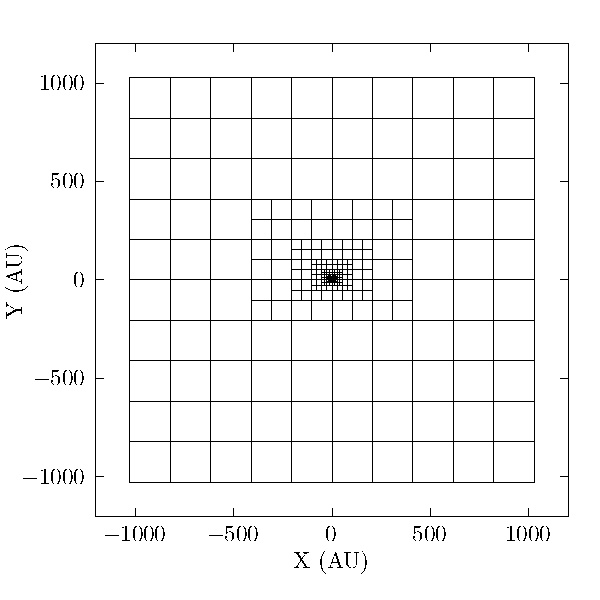
\includegraphics{assets/mesh/gridxy.pdf}
  \caption[Static mesh refinement example]{Plot of blocks used in a 7 level simulation with a block size of $32\times 32 \times 8$ cells. The block density increases dramatically closer to the barycentre.}
  \label{fig:smr-grid}
\end{figure}

The wind outflow from each star is simulated by replacing the conserved variables (density, momentum and energy) within a small region around the expected position of the stars; this region is typically on the order of 6 maximally refined cells in radius.
This rewrite corresponds to a change in mass and mechanical energy imparted by an outflowing wind, such that

\begin{subequations}
  \begin{align}
    \rho_R & = \frac{\dot M}{(4 \pi r^2 v_\infty)} , \\
    p_{R}  & = \rho_R v_\infty , \\
    E_R    & = \frac{P_R}{\gamma - 1} + \frac{1}{2} \rho_{R} v_\infty^2 ,
  \end{align}
\end{subequations}

% This may need more explanation, depending on previous equations
\noindent
where $v_r$ is the wind velocity as it flows radially from the center of the ``remap zone'', $P_R$ is the remap pressure, $P_R = \rho_R k_B T_w / \mu m_H$, $T_w$ is the wind temperature and $r$ is the distance from the current cell to the centre of the remap zone.
Orbits are calculated by moving the remap zones in a manner consistent with Keplerian dynamics, which are updated at every timestep.

% Plasma and dust cooling

\subsection{Gas and dust cooling} \label{sec:gas-dust-cooling}

Cooling due to photon emission from atoms, ions and free electrons, as well as dust particles is simulated by removing energy from a cell at each timestep.
The total energy loss is calculated by integrating the energy loss rates due to gas, plasma and dust cooling using the Euler method; in regions with very rapid cooling sub-stepping is used to improve accuracy, with the number of sub-steps being determined by comparing the substep time to the cooling timescale of the cell.
Gas cooling is simulated using a lookup table method.
A data file containing the gas temperature and associated normalised emissivity, $\Lambda(T)$ of the wind at that temperature is read into the simulation.
In a typical cooling step, the temperature is calculated and a binary search is performed to find the nearest temperature in the lookup table.
A linear interpolation is then performed to find an appropriate value for $\Lambda$.
Energy loss can be calculated with the formulae:

\begin{equation}
  \frac{dE}{dt} = \left(\frac{\rho}{m_H}\right)^2 \Lambda_w(T),
\end{equation}

\noindent
where $\rho$ is the gas density and $m_H$ is the mass of a hydrogen atom.
The lookup table was generated by mixing a series of cooling curves generated by MEKAL simulations of elemental gasses.
These are combined based on the elemental abundances of each wind such that:

\begin{subequations}
  \begin{align}
    \Lambda_\text{WR}(T) & = n_e n_i \sum{X_\text{WR} \Lambda_\text{WR}{E}(T)}, \\
    \Lambda_\text{OB}(T) & = n_e n_i \sum{X_\text{OB} \Lambda_\text{OB}{E}(T)},
  \end{align}
\end{subequations}

\noindent
where $n_e$ and $n_i$ are the electron and ion number density, $X$ is the abundance of an element, and $\Lambda_E(T)$ is the cooling parameter of an element.
Figure \ref{fig:cooling-curve} shows the cooling curves used for each star.
Two lookup tables are used in the simulations, based on the elemental abundances of each star. 
The Wolf-Rayet star uses a curve with abundances typical of a WC9 star with total hydrogen depletion and a high carbon mass fraction, while the OB star is assumed to have solar abundances.
The most significant abundances used in this projects simulations are presented in table \ref{tab:abundances}.
The cooling regime of this code ranges from $10^4$ to $10^9\,\si{\kelvin}$.
A floor temperature of $10^4$ \si{\kelvin} is implemented, temperatures between $\SI{1e4}{\kelvin} < T \leq \SI{1.1e4}{\kelvin}$ are reduced to $10^4\,\si{\kelvin}$ as they are assumed to be either rapidly cooling or a part of the stellar wind.

\begin{table}
  \centering
  \begin{tabular}{@{}ccc@{}}
  \toprule
  \multicolumn{1}{l}{} & \multicolumn{2}{c}{X(E)} \\ \cmidrule(l){2-3} 
   & Solar & WC9 \\ \midrule
  H & $0.705$ & $0.0$ \\
  He & $0.275$ & $0.546$ \\
  C & $3.07 \times 10^{-3}$ & $0.4$ \\
  N & $1.11 \times 10^{-3}$ & $0.0$ \\
  O & $9.60 \times 10^{-3}$ & $0.05$ \\
  % Ne & $1.75 \times 10^{-3}$ & $0.0$ \\
  % Na & $3.47 \times 10^{-5}$ & $3.47 \times 10^{-5}$ \\
  % Mg & $7.10 \times 10^{-4}$ & $7.10 \times 10^{-4}$ \\
  % Al & $6.13 \times 10^{-5}$ & $6.13 \times 10^{-5}$ \\
  % Si & $8.60 \times 10^{-4}$ & $8.60 \times 10^{-4}$ \\
  % S & $3.82 \times 10^{-4}$ & $3.82 \times 10^{-4}$ \\
  % Ar & $1.01 \times 10^{-4}$ & $1.01 \times 10^{-4}$ \\
  % Ca & $6.15 \times 10^{-5}$ & $6.15 \times 10^{-5}$ \\
  % Fe & $1.52 \times 10^{-3}$ & $1.52 \times 10^{-3}$ \\
  % Ni & $7.65 \times 10^{-5}$ & $7.65 \times 10^{-5}$ \\ \bottomrule
  \end{tabular}
  \caption[Abundances used for OB and WR stars]{Abundances used for the OB and WR stars being simulated, other elements are assumed trace when calculating radiative energy loss due to dust.}
  \label{tab:abundances}
\end{table}


\begin{figure}[ht]
  \centering
  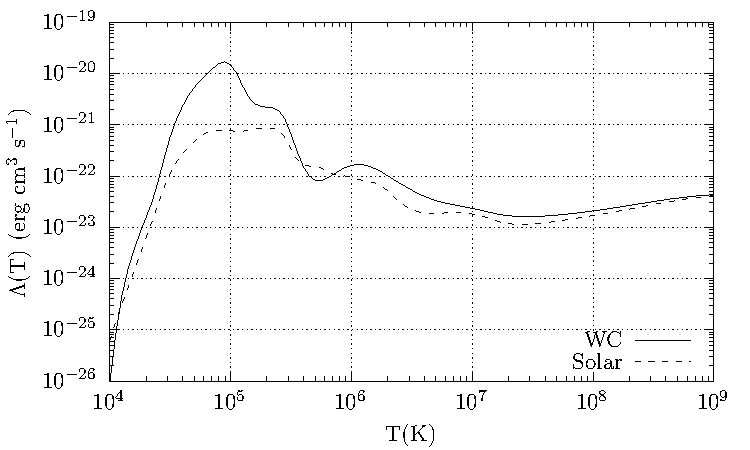
\includegraphics{assets/cooling-curve/cooling-curve-no-elements.pdf}
  \caption[WR and OB $\Lambda(T)$ cooling curves]{Comparison of lookup tables for calculating energy loss due to gas cooling.}
  \label{fig:cooling-curve}
\end{figure}

A model for cooling due to emission from dust grains is also included as dust cooling is expected to play a significant role in the evolution of each system.
The rate of cooling is calculated using the uncharged particle case of the \textcite{dwek_infrared_1981} prescription.
Grains are heated due to collisions with ions and electrons, causing them to radiate, with energy being removed from the simulation.
This assumes that the region being simulated is optically thin to far infrared photons.
The energy loss rate is calculated with the following formulae:

\begin{subequations}
  \begin{align}
    H_\text{coll} & = 1.26 \times 10^{-19} \frac{n}{A^{1/2}} a^2(\mu \text m) T^{3/2} h(a,T) , \\
        \Lambda_d & = \frac{H_\text{coll} + H_\text{el}}{n_H} , \\
    \frac{dE}{dt} & = n_T n_d \Lambda_d ,
  \end{align}
\end{subequations}

\noindent
where $H_\text{coll}$ is the heating rate due to atom and ion collisions, $H_\text{el}$ is the heating rate due to electron collisions, $h(a,T)$ is the grain-ion transparency and $n_T$ is the total ion number density.
$H_\text{coll}$ is summated for Hydrogen, Helium, Carbon, Nitrogen and Oxygen atom collisions.
Other elements are not considered as they are present in trivial proportions in both winds.

\begin{figure}[h]
  \centering
  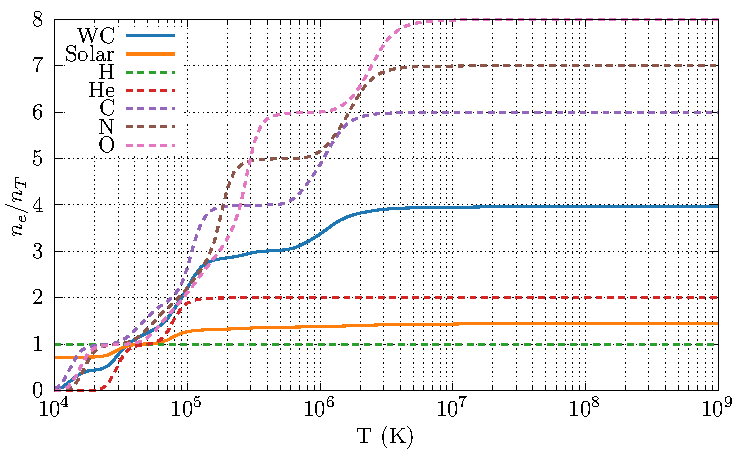
\includegraphics{assets/ionisation-fraction/ionisation-fraction.pdf}
  \caption[OB and WR electron-ion ratios]{A comparison of the electron-ion ratio of both winds as the temperature changes. Included are the pure wind flows that the lookup tables are built from.}
  \label{fig:electron-curve}
\end{figure}

Electron-grain collisions are modelled similarly to ions, albeit with some differences.
One major factor for calculating accurate energy loss due to electron collisions is that the electron number density needs to be accurately calculated; this is performed with a second series of lookup tables that contain the electron-to-ion ratio of each wind across a temperature range of $10^4$ to $10^9\si{\kelvin}$ (figure \ref{fig:electron-curve}).
The electron number density is found to be $n_e = \beta n_i$ where $\beta$ is the electron-to-ion ratio and $n_i$ is the ion number density.
Another difference between calculating electron-grain and gas-grain cooling is calculating electron-grain transparency, which is a significantly more complex problem than calculating ion-grain transparency.
An assumed full opacity proves to be extremely inaccurate at temperatures $>10^6$ \si{\kelvin}.
Electron-grain transparency is therefore calculated via an approximation described in \textcite{dwek_infrared_1981}:

\begin{equation}
  \begin{alignedat}{3}
    h(x^*) & = 1 ,                && ~~ x^* > 4.5, \\
           & = 0.37{x^*}^{0.62} , && ~~ x^* > 1.5 , \\
           & = 0.27{x^*}^{1.50} , && ~~ \text{otherwise,}
  \end{alignedat}
\end{equation}

\noindent
where $x^* = \num{2.71e8} a^{2/3} (\si{\micro\metre})/T$.
This approximation is approximately 4 orders of magnitude faster than using an integration method, while only being out by $\sim 8\%$ in the worst case scenario (figure \ref{fig:lambdacomparison}).
Grain-grain collisions are not modelled, as this would be difficult to calculate due to the single-fluid model in use.
Further simulations utilising a multi-fluid model could allow for this to be simulated.

\begin{figure}
  \centering
  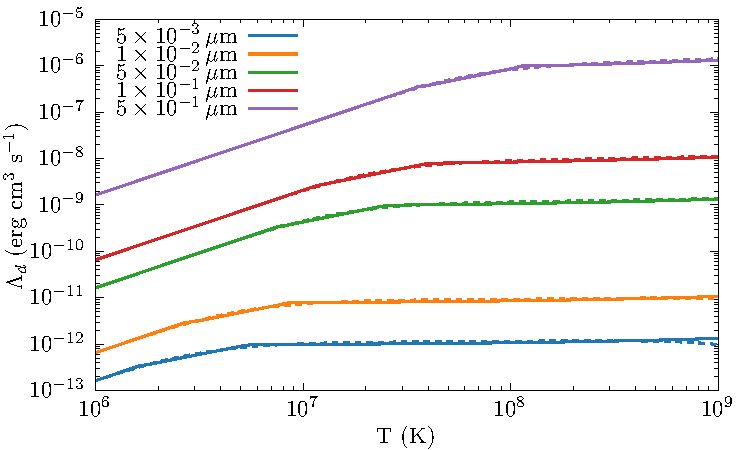
\includegraphics{assets/grain-transparency/lambda-comp.pdf}
  \caption[Comparison of electron transparency methods.]{$\Lambda_d$ as a function of temperature for various grain sizes. The estimate method is extremely close to the integral value aside from at the highest temperatures.}
  \label{fig:lambdacomparison}
\end{figure}

\subsection{Numerical modelling of dust through advected scalars}

The most important modification to Athena++ was the addition of a dust growth and destruction model to simulate the production of dust within the WCR.
A passive scalar model was used where dust can evolve and advect through the simulation, analogous to a co-moving fluid, which previous papers have noted is an accurate dynamical model for dust within the WCR \parencite{hendrix_pinwheels_2016}.
In these simulations, dust is stored in the form of two variables, the average grain radius, $a$, and the dust-to-gas mass ratio, $z$.
From these constants the dust production rate, number density, and total dust mass can be derived.
A co-moving model allows for a simplified model of dust formation. In such a model, the mean particle velocity between two particles of different size can be given as:

\begin{equation}
  \langle u \rangle = \left[ \frac{8kT}{\pi m_r} \right] ^{1/2} ,
\end{equation}

\noindent
where $m_r$ is the familiar reduced mass between a test particle of mass $m_t$ and a field particle of mass $m_f$

\begin{equation}
  m_r = \frac{m_f m_t}{m_f + m_t} .
\end{equation}

\noindent
As the dust grain is significantly more massive, the reduced mass is approximately equal to the grain mass, simplifying the dynamics of the simulation in a co-moving case.
Dust growth is modelled through approximating growth due to grain-gas accretion where grains co-moving with a gas perform relatively low-velocity collisions with the surrounding gas, causing it to accrete onto the surface of the dust grain \parencite{spitzer_jr._physical_2008}.
Assuming a single average grain size the change in average grain radius is given by

\begin{equation}
  \frac{da}{dt} = \frac{\xi_a \rho_{Gr} w_a}{4 \rho} ,
\end{equation}

\noindent
where $w_a$ is the Maxwell-Boltzmann distribution RMS velocity, $\xi_a$ is the grain sticking efficiency and $\rho_{Gr}$ is the grain bulk density.
The associated rate of dust density change is found to be

\begin{equation}
  \frac{d\rho_D}{dt}  = 4 \pi a^2 \rho_g n_D \frac{da}{dt} , 
\end{equation}

\noindent
where $\rho_g$ is the gas density and $n_D$ is the grain number density.
In this paper $\xi_a$ is assumed to be $10\%$ while a bulk density analogous to amorphous carbon grains of $3 \, \si{g.cm^{-3}}$ is utilised.

Dust destruction is calculated via gas-grain sputtering using the \textcite{draine_destruction_1979} prescription - a dust grain has a lifespan, $\tau$, which is dependent on the grain radius.
Assuming a spherical grain, the rate of change in mass and radius can be calculated such that:

\begin{subequations}
  \begin{align}
           \tau_D & = 1 \, \text{Myr} \times \frac{a}{n_g} , \\
    \frac{da}{dt} & = - \frac{a}{\tau_D} , \\
    \frac{dm}{dt} & = -1.33 \times 10^{-13} a^2 n_g n_d \rho_{Gr} ,
  \end{align}
\end{subequations}

\noindent
where $n_g$ is the gas number density.

% //TODO cleanup sentence structures

In order to propagate dust through each simulation, a small initial value for the advected scalars is set in each cell in the remap zones.
A minimum grain radius of $50 \, \text{\AA}$ and minimum dust-to-gas mass ratio of $10^{-8}$ is imposed.
Changing $z_{min}$ does not significantly impact the final dust-to-gas mass ratio of the system as $z$ rapidly increases within the WCR and dust growth in the WCR dominates the total production.

\section{Model Parameters}

In this paper we do not intend on modelling particular systems.
Rather we intend to gain a deeper understanding of what the primary influences of dust formation are in a CWB system.
A series of simulations were therefore run in order to determine how dust formation varies due changes in orbital separation and wind momentum ratio.
A baseline simulation with properties similar to WR98a with a circular orbit and identical stellar masses was created.
Additionally, this baseline simulation has a momentum ratio of $0.02$.
Other simulations were then run with different orbital separations and/or wind momentum ratios.
Another set of simulations were run where the cooling mechanisms were selectively disabled, in order to understand how radiative cooling effects the dust production rate.
Table \ref{tab:baseline-windproperties} and \ref{tab:baseline-orbits} detail the wind and orbital parameters of the baseline simulation.
The orbital separation is modified by changing the orbital period of the simulation, while wind momentum ratio is modified by adjusting the mass loss ratio and wind terminal velocity for each star.
Two simulation sub-sets for this were performed, simulations where the wind terminal velocities were adjusted for each star and simulations where the mass loss rates for each star were adjusted.

\begin{table}
  \centering
  \begin{tabular}{cccc}
  \hline
  Parameter & WR & OB & Unit \\ \hline
  $\dot M$ & \num{5.0e-6} & \num{5.0e-8} & \si{\solarmass\per\year} \\
  $v_\infty$ & \num{1.0e8} & \num{2.0e8} & \si{cm.s^{-1}} \\
  $T_w$ & \num{1.0e4} & \num{1.0e4} & K \\
  \hline
  \end{tabular}
  \caption{Wind properties of the baseline system.}
  \label{tab:baseline-windproperties}
\end{table}

\begin{table}
  \centering
  \begin{tabular}{ccc}
  \hline
  Parameter & Value & Unit \\ \hline
  $M$ & 10.0 & \si{\solarmass} \\
  $d_{sep}$ & \num{4.0} & \si{\au} \\
  $P$ & \num{1.80} & \si{\year} \\
  \hline
  \end{tabular}
  \caption{Baseline system orbital properties.}
  \label{tab:baseline-orbits}
\end{table}

\subsection{Cooling mechanisms}

For this set of simulations, the influence of cooling was changed by varying how cooling works within the simulations.
All simulations in this set keep the same orbital and wind parameters, which are that of the baseline system described in tables \ref{tab:baseline-windproperties} \& \ref{tab:baseline-orbits}.
One simulation has both plasma and dust cooling in operation (the \texttt{fullcool} simulation), while the other two simulations have plasma cooling only and no cooling respectively (\texttt{plasmacool} and \texttt{nocool}, table \ref{tab:cooling-param}).
The final, no radiative cooling simulation instead relies on adiabatic expansion for temperature change; as such, this simulation behaves as if it has a $\chi$ value for both winds that is arbitrarily high.
The post-shock flow in the \texttt{nocool} model will also be unable to compress as much due to the lack of energy loss via radiative cooling.
The role of these simulations is to discern whether it is cooling alone or other system parameters that affects dust production.

% Discuss why this is important, mention overdensity due to radiative cooling

\begin{table}
  \centering
  \begin{tabular}{ccc}
    \hline
    Name & Plasma cooling & Dust cooling \\
    \hline
    \texttt{fullcool} & Yes & Yes \\ 
    \texttt{plasmacool} & Yes & No \\
    \texttt{nocool} & No & No \\
    \hline
  \end{tabular}
  \caption{Cooling series simulation parameters}
  \label{tab:cooling-param}
\end{table}

\subsection{Wind momentum ratio}

Another set of simulations was devised in order to assess the influence of the wind parameters on the formation of dust within a CWB.
As the wind momentum ratio is dependent on both the mass loss rate and wind velocity of each star, each of these properties is modified over a course of simulations.
$\eta$ is varied from 0.01 to 0.04 by adjusting the wind parameters for each star.
This is further subdivided by which property is modified, either the mass loss rate (table \ref{tab:mdot-param}) or wind terminal velocity (table \ref{tab:vinf-param}).
As the cooling parameter has a much stronger dependency on $v_\infty$ than $\dot{\text{M}}$, the modification of either parameter while maintaining a similar value for $\eta$ allows us to determine whether the cooling parameter is the primary characteristic determining the formation of dust within WCd systems.
This can be seen when comparing simulations \texttt{mdot-1} and \texttt{vinf-1}, which have similar wind momentum ratios but the cooling parameters for the WC star differ by a factor of 32.
These simulations are compared to the baseline simulation, which a radiative post-shock WCR.
Whilst the simulations with $\eta = 0.00$ still have very imbalanced winds, they are typical of a WR+OB binary with a less intense Wolf-Rayet partner star wind.
All simulations were run for a minimum of 1 orbit.
As these orbits are circular, there should be no major variance of the winds after the start-up transients are fully advected, save for some fluctuations.

\begin{table}
  \centering
  \begin{tabular}{ccccccc}
  \hline
  Name & $\dot M_{WR}$ & $\dot M_{OB}$ & $v^\infty_{WR}$ & $v^\infty_{OB}$ & $\eta$ & $\chi_{WR}$ \\ 
  & \si{\solarmass\per\year} & \si{\solarmass\per\year} & \si{\centi\metre\per\second} & \si{\centi\metre\per\second} & & \\ \hline
  \texttt{baseline}& \num{5.0e-6} & \num{5.0e-8} & \num{1e8} & \num{2e8} & 0.02 & 1.049 \\
  \texttt{mdot-1}  & \num{1.0e-5} & \num{5.0e-8} & \num{1e8} & \num{2e8} & 0.01 & 0.544 \\
  \texttt{mdot-2}  & \num{2.5e-6} & \num{5.0e-8} & \num{1e8} & \num{2e8} & 0.04 & 1.995 \\
  \texttt{mdot-3}  & \num{5.0e-6} & \num{1.0e-7} & \num{1e8} & \num{2e8} & 0.04 & 0.997 \\
  \texttt{mdot-4}  & \num{5.0e-6} & \num{2.5e-8} & \num{1e8} & \num{2e8} & 0.01 & 1.088 \\
  \hline
  \end{tabular}
  \caption[Mass loss rate series wind parameters]{Wind parameters for simulations varying the mass loss rate, $\dot M$.}
  \label{tab:mdot-param}
\end{table}

\begin{table}
  \centering
  \begin{tabular}{ccccccc}
  \hline
  Name & $\dot M_{WR}$ & $\dot M_{OB}$ & $v^\infty_{WR}$ & $v^\infty_{OB}$ & $\eta$ & $\chi_{WR}$ \\ 
  & \si{\solarmass\per\year} & \si{\solarmass\per\year} & \si{\centi\metre\per\second} & \si{\centi\metre\per\second} & & \\ \hline
  \texttt{baseline} & \num{5e-6} & \num{5e-8} & \num{1e8} & \num{2e8} & 0.02 & 1.049 \\
  \texttt{vinf-1}   & \num{5e-6} & \num{5e-8} & \num{2e8} & \num{2e8} & 0.01 & 17.41 \\
  \texttt{vinf-2}   & \num{5e-6} & \num{5e-8} & \num{5e7} & \num{2e8} & 0.04 & 0.062 \\
  \texttt{vinf-3}   & \num{5e-6} & \num{5e-8} & \num{1e8} & \num{4e8} & 0.04 & 0.997 \\
  \texttt{vinf-4}   & \num{5e-6} & \num{5e-8} & \num{1e8} & \num{1e8} & 0.01 & 1.088 \\
  \hline
  \end{tabular}
  \caption[Terminal velocity series wind parameters]{Wind parameters for simulations varying the wind terminal velocity, $v^\infty$.}
  \label{tab:vinf-param}
\end{table}

\subsection{Separation distance}

A final series of simulations was performed with the wind parameters equivalent to the baseline model, but with differing orbital separations.
The separation was altered by modifying the orbital period of each star, as stellar masses were to be kept realistic.
The separation distance was varied from the baseline model of 4 \si{\au} to 64 \si{\au} (table \ref{tab:dsep-param}), which has the effect of modifying the cooling parameter of each simulation without changing the wind momentum ratio; allowing us to further discern which is the dominant parameter influencing dust formation.
For instance, simulation \texttt{dsep-64AU} has a cooling parameter value approaching the fast WR wind model \texttt{vinf-1}, despite having a wind momentum ratio of 0.02.

%//TODO this section needs some analytical work, specifically on the expected values for dt, things like that, I can also get some stuff from the results
Each simulation has a coarse resolution of $320 \times 320 \times 40$ cells, with a varying number of levels, as the separation distance is doubled, the associated static mesh refinement box is halved and the number of levels is decremented. This manipulation of levels ensures that the number of cells between the stars is kept consistent, reduces memory usage and keeps the average timestep approximately the same.
Similarly to the previous set of simulations, a minimum of 1 orbit was needed for each simulation, however, as the orbital period of each simulation varies, certain simulations were able to run for a significantly longer length of time, with data for multiple orbits being obtained.

\begin{table}[h]
  \centering
  \begin{tabular}{cccccc}
    \hline
    Name & P & $d_{sep}$ & $\chi_{WR}$ & Levels & Effective Resolution \\
    & \si{\second} & \si{\au} &  &  & Cells \\ \hline 
    \texttt{dsep-4AU}  & \num{1.80} & 4  & 1.05 & 7 & $20480 \times 20480 \times 2560$ \\
    \texttt{dsep-8AU}  & \num{5.06} & 8  & 2.10 & 6 & $10240 \times 10240 \times 1280$ \\
    \texttt{dsep-16AU} & \num{14.3} & 16 & 4.19 & 5 & $5120 \times 5120 \times 640$    \\
    \texttt{dsep-32AU} & \num{40.5} & 32 & 8.39 & 4 & $2560 \times 2560 \times 320$    \\
    \texttt{dsep-64AU} & \num{115}  & 64 & 16.8 & 3 & $1280 \times 1280 \times 160$    \\ \hline
  \end{tabular}
  \caption{Parameters of simulations varying separation distance.}
  \label{tab:dsep-param}
\end{table}

\subsection{Data collection}

Data was collected in multiple forms.
HDF5 files were generated at regular time intervals - 3D HDF5 meshes were generated every $1/100^{\text{th}}$ of an orbit, while 2D slices were produced every $1/1000^{th}$ of an orbit.
These HDF5 files contain the primitive variables of the simulation, gas density, $\rho$, gas pressure, $P$ and wind velocity components, $v_x$, $v_y$ and $v_z$; these can be used to derive other variables such as the gas temperature as well as the internal, kinetic and total energies.
The scalars governing the dust properties were also stored for each cell, the dust-to-gas mass ratio, $z$ and the dust grain radius, $a$.
The wind ``colour'' was also tracked.
This is the proportion of gas resultant from each star; a value of 1.0 is a pure WR wind, 0.0 is a pure OB wind, while 0.5 is a perfectly mixed wind.
In addition to HDF5 outputs, the volume-weighted summations of all system parameters, such as the total system mass and summated average grain radius were collected.
In order to derive average values, such as $\bar{z}$ and $\bar{a}$, the values for each can be divided by the total system mass.
To calculate dust formation within the WCR, a method of determining if a cell was a part of the wind collision region was devised - the cell density would be compared to the predicted density of a single smooth wind with the wind parameters of the Wolf-Rayet star in the system:

\begin{equation}
  \rho_\text{SW} = \frac{\dot{M}_{WR}}{4 \pi r^2 v^\infty_{WR}},
\end{equation}

\noindent
where $r$ is the distance from the barycentre. This threshold value was set to $1.25\rho_\text{SW}$ as it most accurately determined if a cell was part of the WCR.
Increased threshold values were not accurate at large distances from the barycentre (figure \ref{fig:overdensity-threshold}).
Other methods of detecting the Wind Collision Region such as determining wind mixing levels were not successful in general.
A mixed wind model for detecting over-density was also considered, however it was not any more accurate than the single wind over-density model. 

\begin{figure}
  \centering
  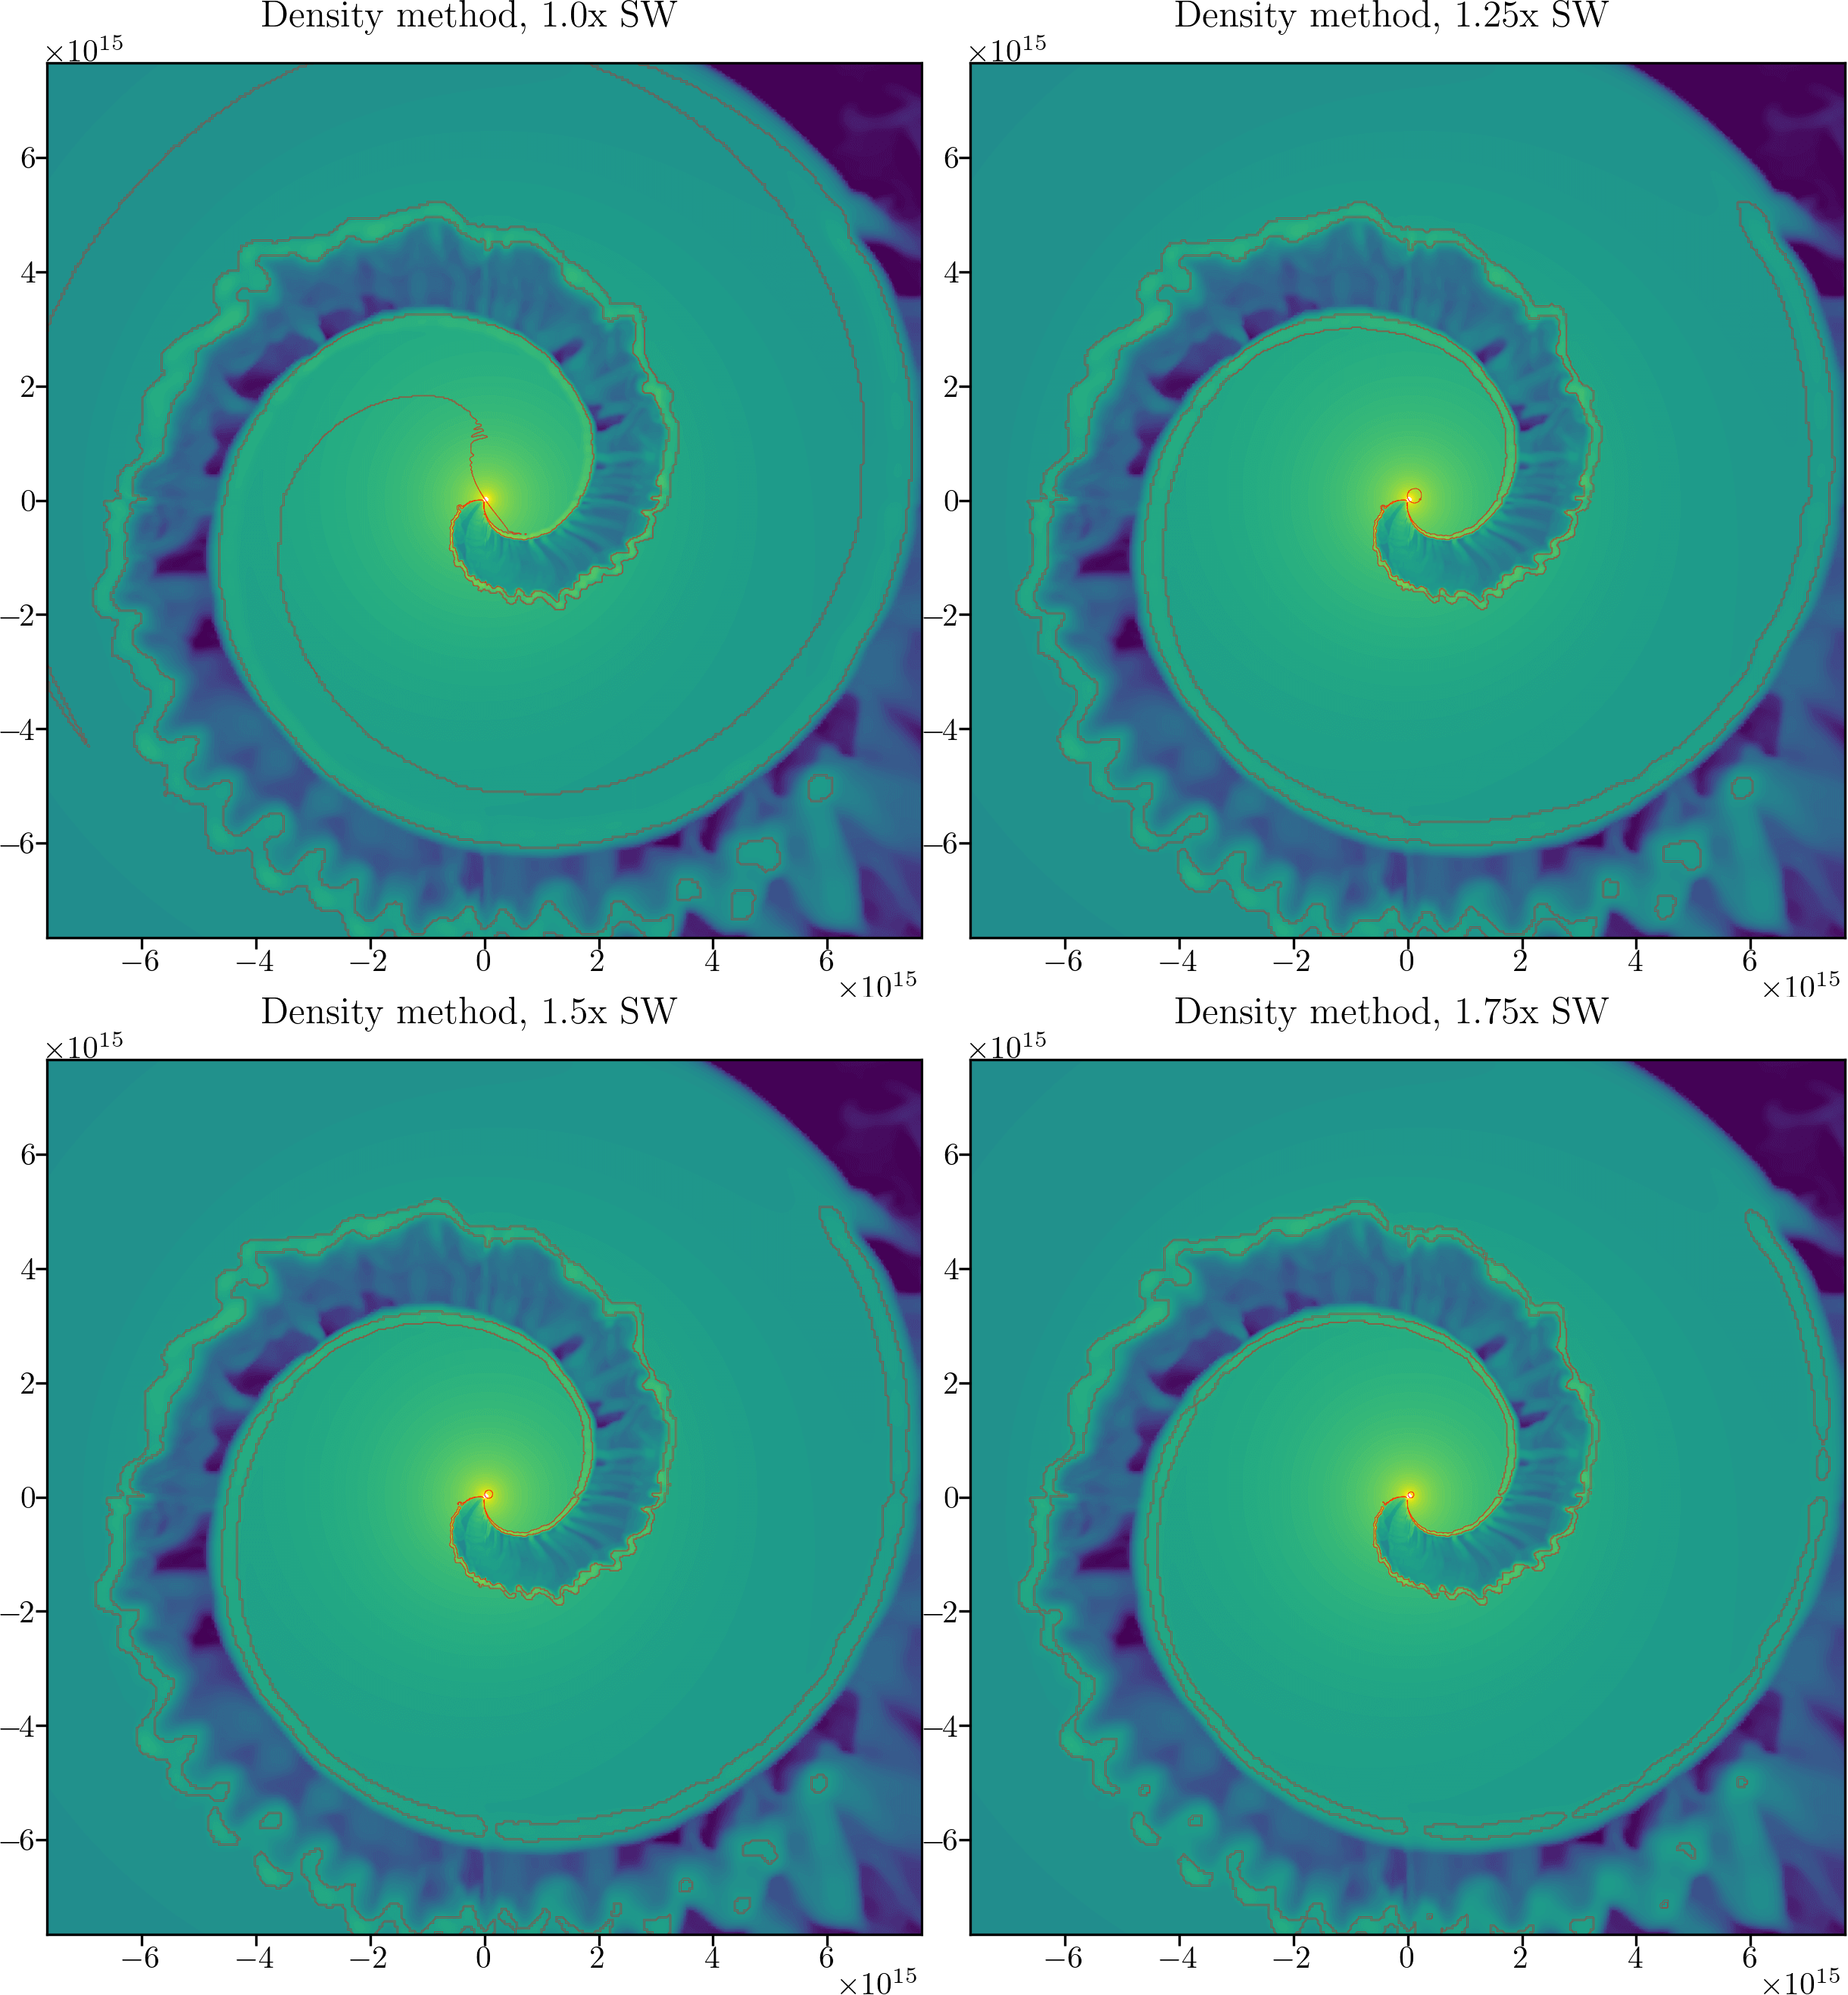
\includegraphics[width=5in]{assets/overdensity-method.png}
  \caption[Comparison of threshold values for over-density method]{Comparison of threshold values for the over-density method of determining if a cell resides in the wind collision region.
  A threshold value of $1.25\rho_\text{SW}$ was chosen as it most accurately determined if the cell was in the post-shock region.}
  \label{fig:overdensity-threshold}
\end{figure}

\section{Results}

\subsection{Radiative processes}

\subsection{Momentum ratio variation}

\subsection{Separation variation}

% % Adiabatic flow 

% The most immediately apparent result to this 

% %//FIXME this needs work! 32AU result is instead labelled as 64AU and zooms aren't consistent!

% \begin{figure}
%   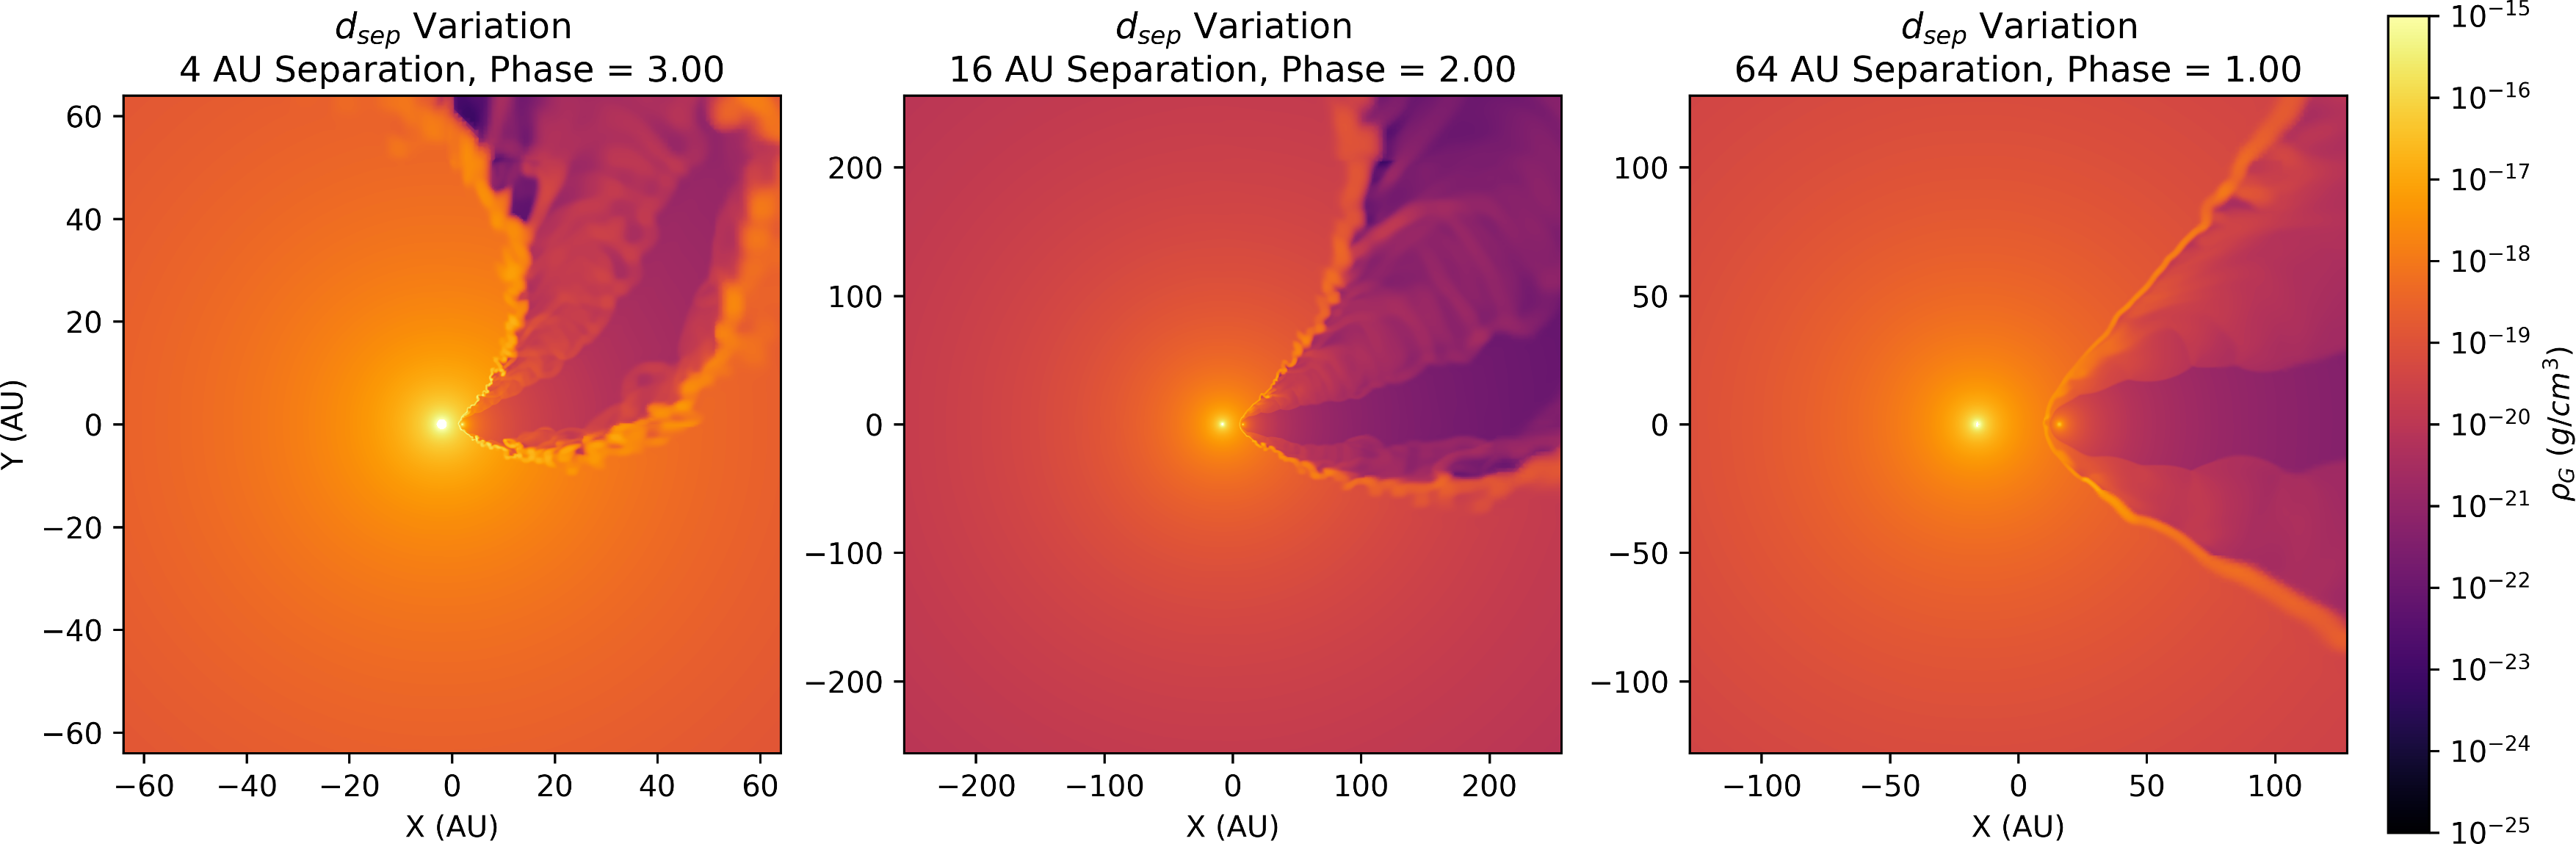
\includegraphics[width=\textwidth]{assets/adiabatic-flow/adiabatic-flow-a4.png}
% \end{figure}

% % Dust yields

% A clear trend with orbital separation is that dust formation increases drastically as the stars are positioned closer together, at high degrees of separation dust formation ceases, and average grain size drops below the initial value of $50 \text \AA$.

% The bulk of dust growth occurs in the immediate post shock region, as dust is rapidly cooled and at a high enough density for dust formation to occur.

% This matches observations of episodic dust forming systems, where infrared emission due to dust is maximised at or shortly after periastron passage. This also lends further evidence that dust formation rates are not influenced solely by the momentum ratio, as this is kept constant, and instead is strongly influenced by the wind density at collision and post-shock cooling. 

% % Periodicity

% Closer orbits were also observed to cause subtle periodic changes, whilst this effect is less pronounced than in a highly eccentric system, the 


% \subsection{Wind mixing within the WCR}

% %This may need additional work

% While interaction between Hydrogen and dust grains is not simulated by the dust model, \cite{leteuffModelDustFormation2002} notes that Hydrogen could be a potential catalyst for amorphous carbon grain formation.


% \appendix
% \section{Derivation of Dust Accretion and Destruction Rates}\label{app:accretiondestruction}

% \subsection{Dust destruction}\label{app:destruction}
